\chapter{User interfaces design}
\section{Mockups}
Some mockups have been already included in the RASD document of PowerEnJoy, in section 3.1.1.
In addition to them we provide other mockups to show other functionalities of the application.

\subsection{Activation of the car}

\begin{figure}[H]
\centering
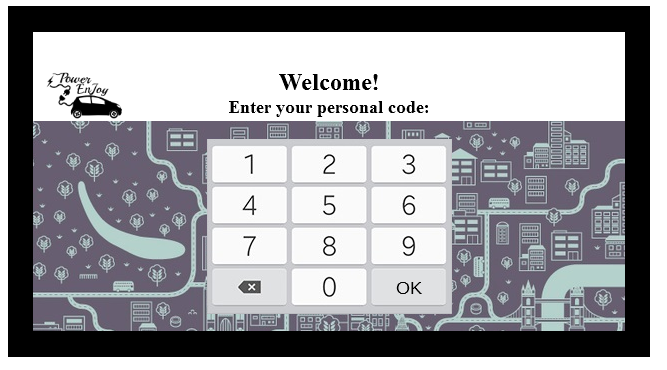
\includegraphics[scale=0.65, keepaspectratio]{../images/mockups/pin.png}
\caption{Activation of the car mockup}
\end{figure}

Once in the car the Client has to insert his/her personal code in order to activate the car.
If she/he doesn’t insert the correct pin he/she won’t be able to ignite the engine.
\subsection{Additional functionalities}

\begin{figure}[H]
\centering
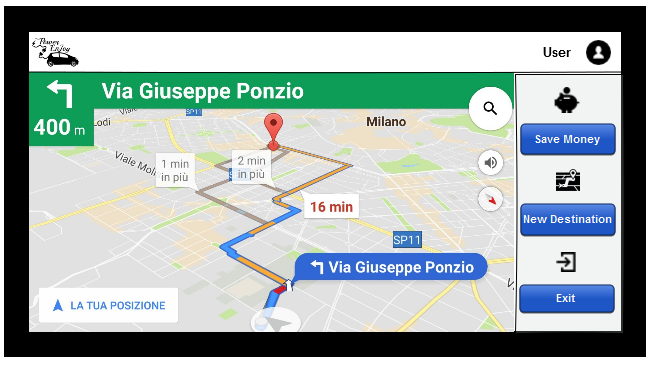
\includegraphics[scale=0.65, keepaspectratio]{../images/mockups/ride.png}
\caption{Additional functionalities mockup}
\end{figure}

When the engine ignites, the GPS navigation device offers the Client the opportunity to use the navigation system and in addition to enable the save money option, in order to obtain a discount.

\subsection{Terminate rent}
\begin{figure}[H]
\centering
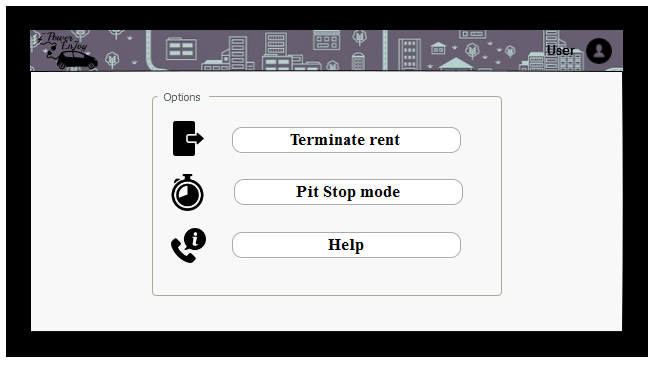
\includegraphics[scale=0.65, keepaspectratio]{../images/mockups/terminate_rent.png}
\caption{Terminate rent mockup}
\end{figure}

The GPS navigation device shows as default this screen, allowing the Client to terminate the rent or to choose the ‘Pit Stop’ mode.
If the Client is using the navigation system, he/she can reach this screen with a click on the exit button(See 4.1.2).

\section{UX diagrams}
The following UX diagram describes paths that a user can follow.
Starting from the homepage of the application (both web and mobile application), a user can choose to do a registration or to login into the system, if he/she has already valid access credentials.
In both cases if an error occurs, for example due to mistaken information, there is an error screen that report to the user that something goes wrong and redirect him/her to a safe screen to redo all the operations.
Once a Registered Client is logged into the system he/she can reserve a car, choosing the address in which he/she wants to look for a car or deciding to be located through the GPS signal of the device.
Then the Registered Client is directed to the Map screen in which he/she can choose a car to rent and once the decision is made he/she return to the Reservation screen.
Then he/she can check the Show Reservation screen, in which there are a recap of the reservation and the possibility to cancel it.

\begin{figure}[H]
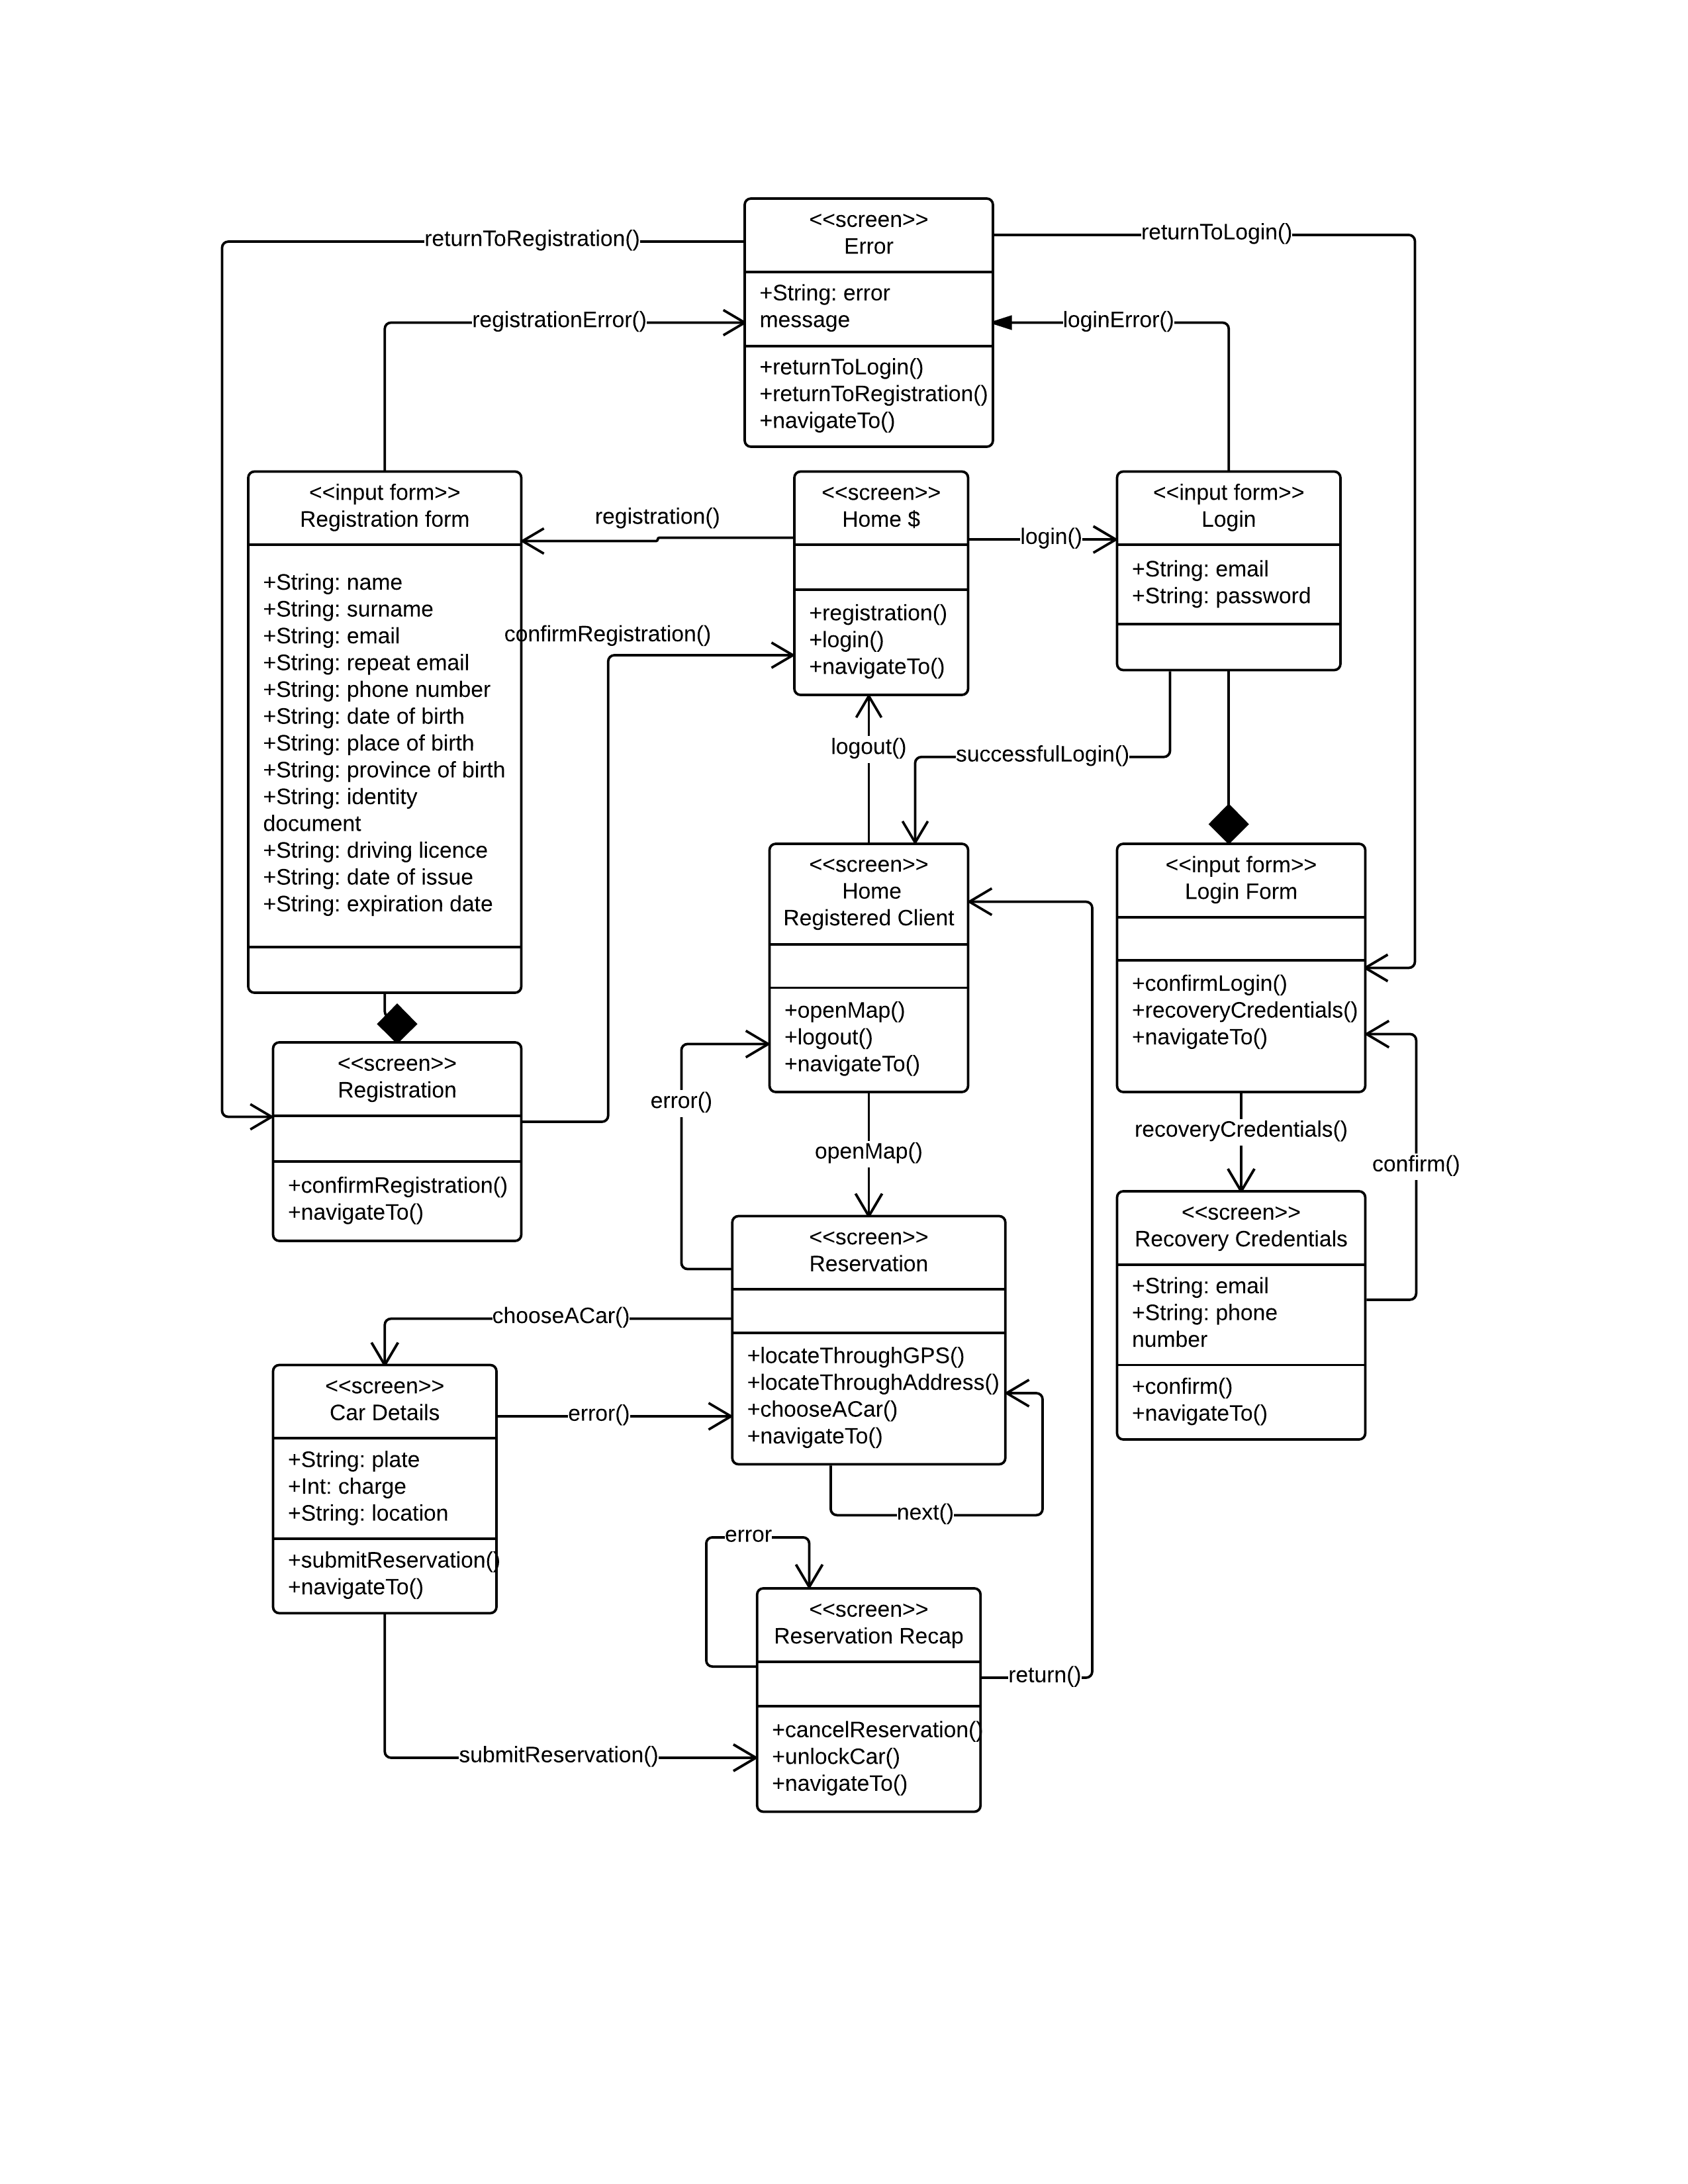
\includegraphics[width=\textwidth, keepaspectratio]{../images/diagrams/ux.png}
\caption{UX diagram}
\end{figure}

\section{BCE diagrams}
The following diagram represents the BCE diagram and shows how a user action, performed on its UI, is managed within the component of our system.

\begin{figure}[H]
\centering
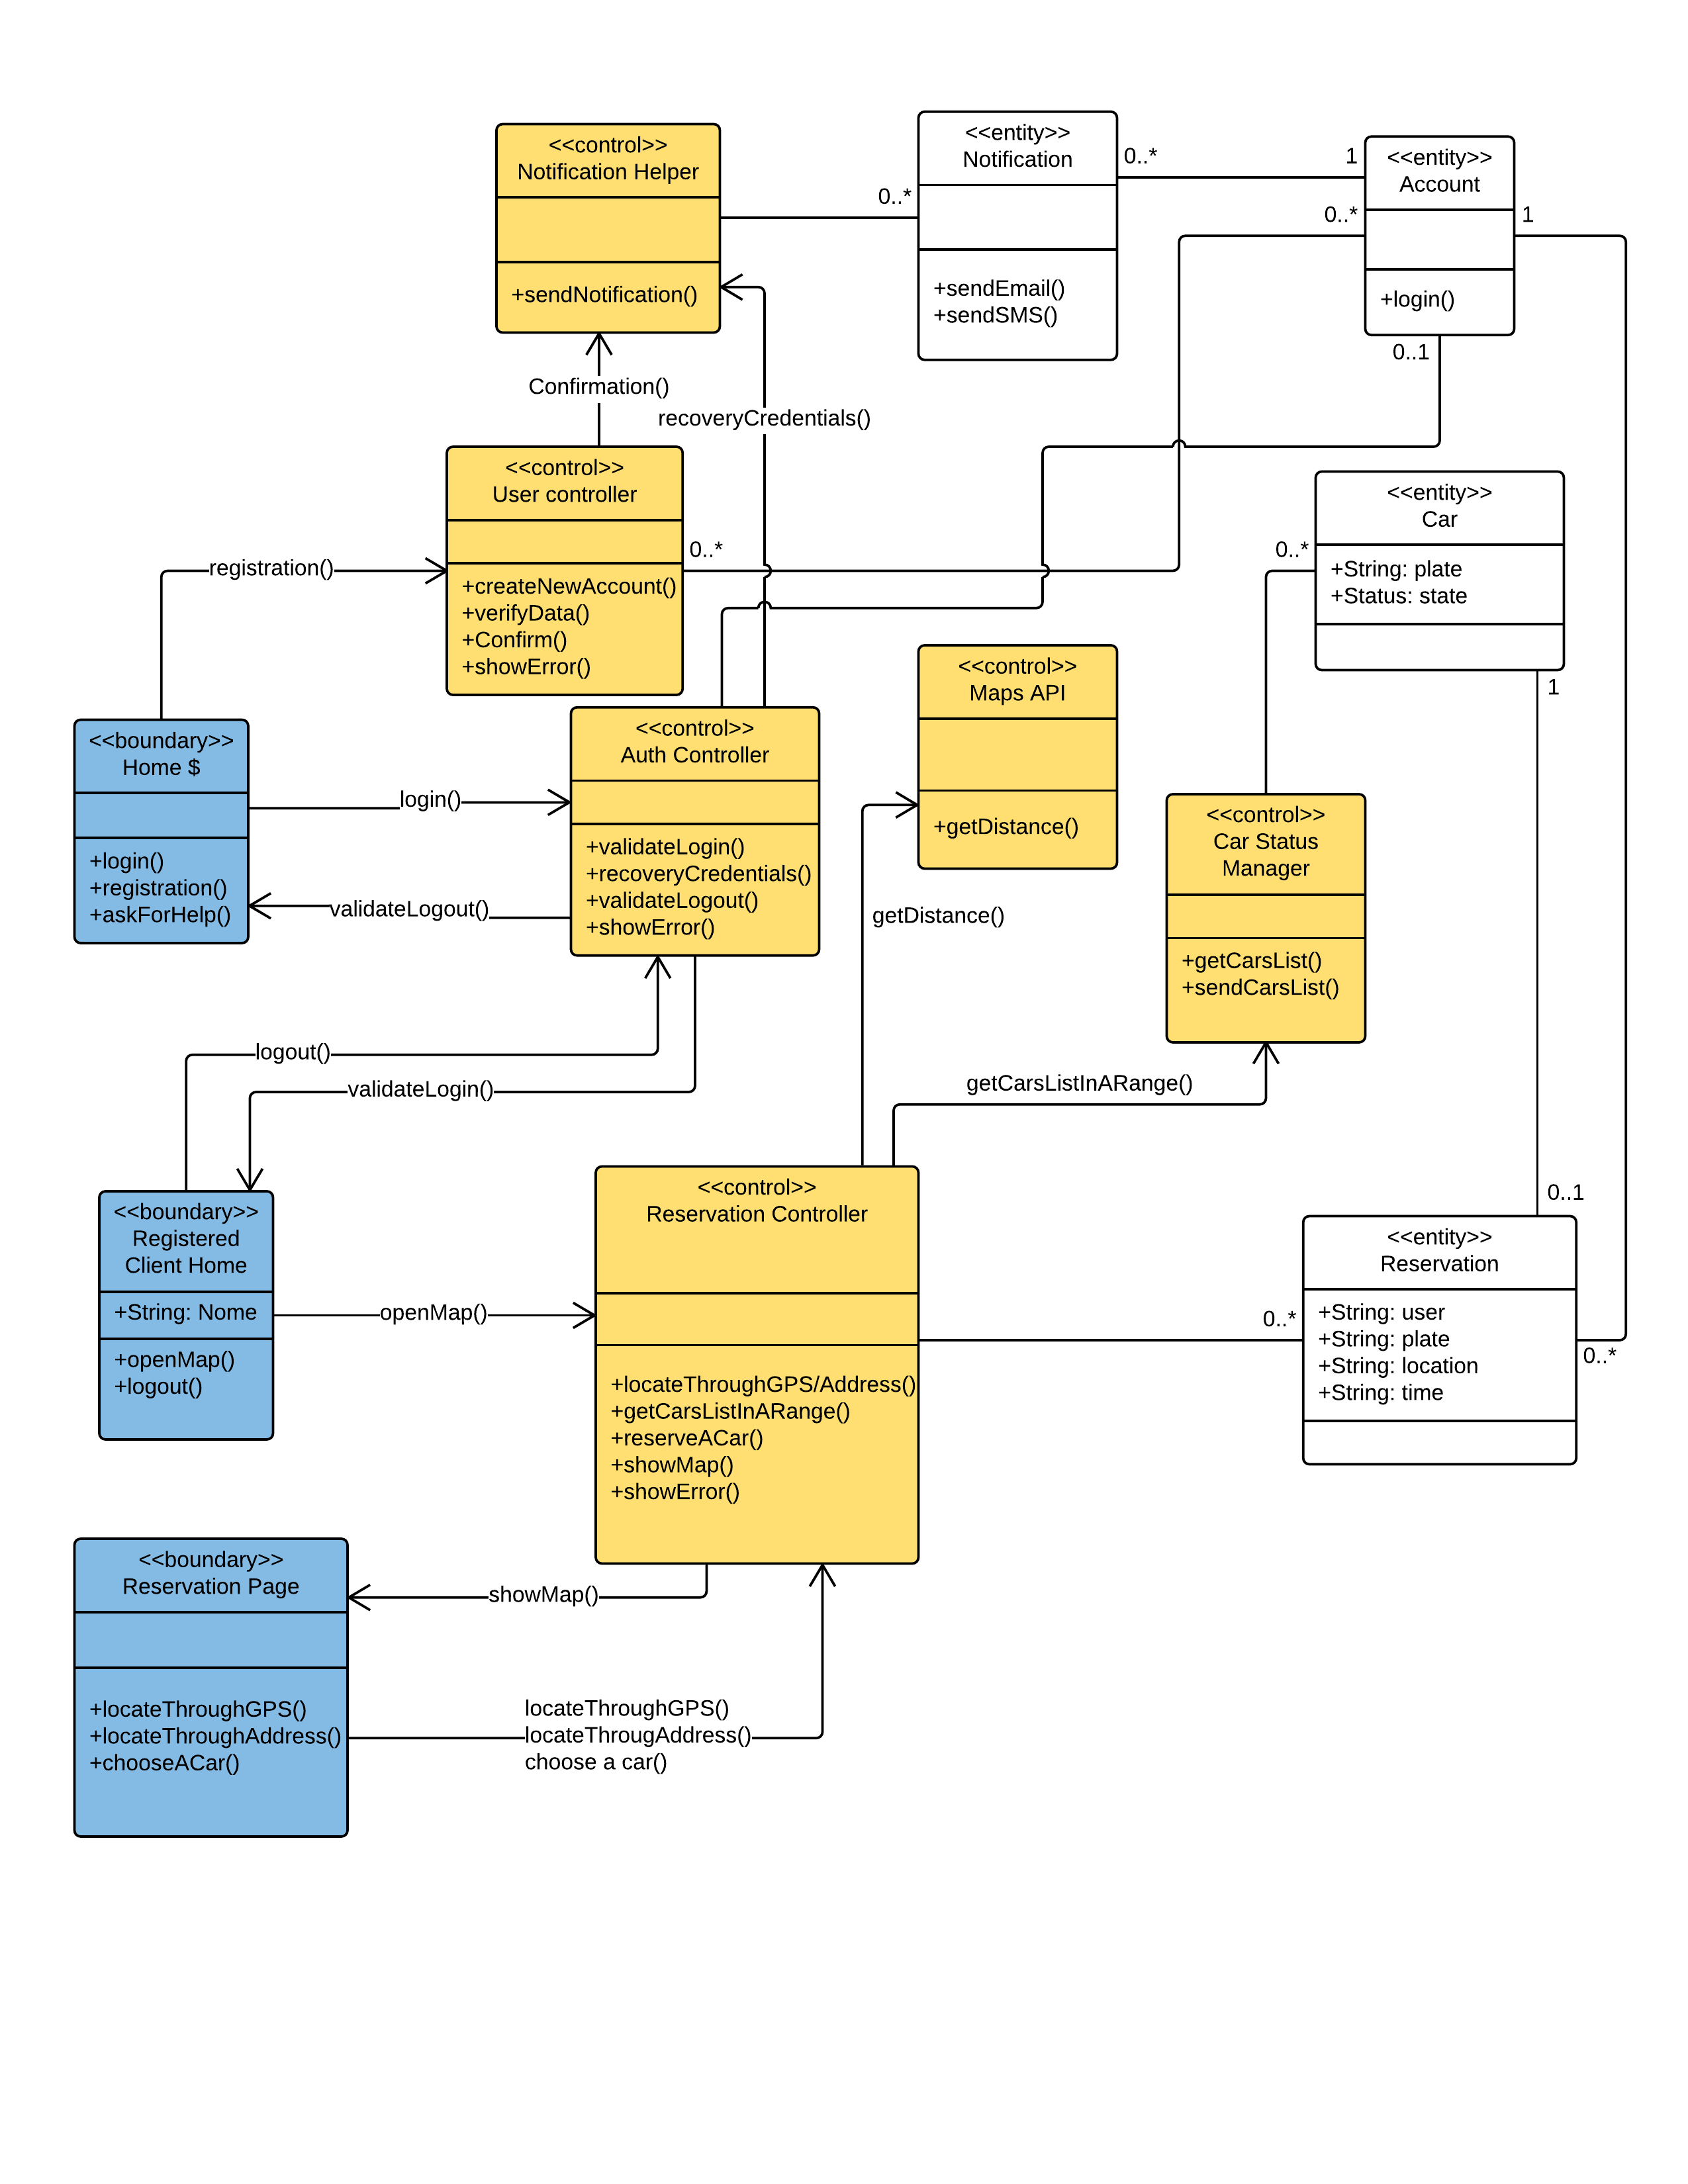
\includegraphics[scale=0.6,keepaspectratio]{../images/diagrams/bce.png}
\caption{BCE diagram}
\end{figure}

